\documentclass{article}
\usepackage{listings}
\usepackage{xcolor}
\usepackage{caption}
\usepackage{float}
\usepackage{tikz}
\usepackage{amsmath}

\begin{document}

\begin{figure}[H]
    \centering
    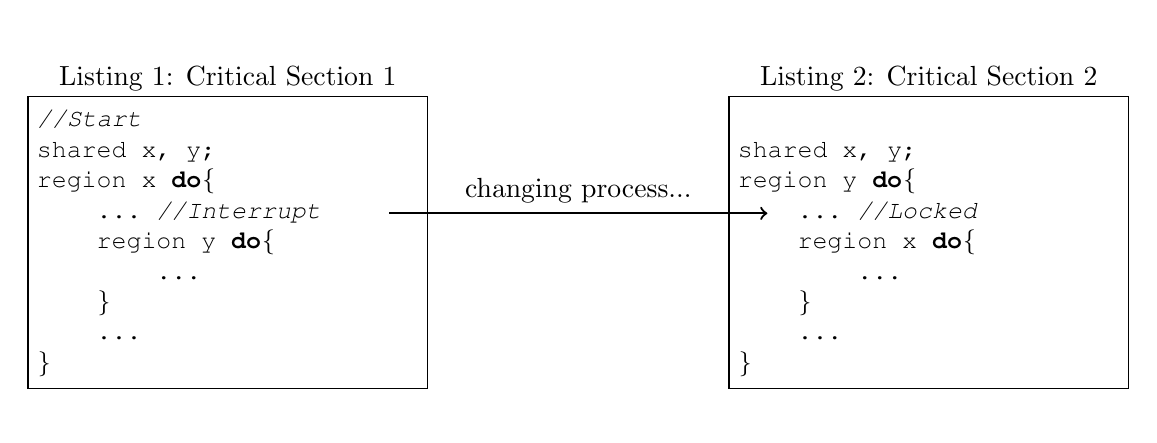
\begin{tikzpicture}
        % Define two minipages for the code blocks
        \node[anchor=north west] (A) at (0, 0) {
            \begin{minipage}{0.40\textwidth}
                \begin{lstlisting}[language=C, caption={Critical Section 1}, basicstyle=\fontfamily{pcr}\selectfont\small, frame=single]
//Start                
shared x, y;
region x do{
    ...	//Interrupt
    region y do{
        ...
    }
    ...
}
                \end{lstlisting}
            \end{minipage}
        };
        
        \node[anchor=north east] (B) at (14, 0) {
            \begin{minipage}{0.40\textwidth}
                \begin{lstlisting}[language=C, caption={Critical Section 2}, basicstyle=\fontfamily{pcr}\selectfont\small, frame=single]
                
shared x, y;
region y do{
    ...	//Locked
    region x do{
        ...
    }
    ...
}
                \end{lstlisting}
            \end{minipage}
        };
        
        % Draw an arrow between the code blocks
        \draw[->, thick] ([xshift=-0.5cm,yshift=0.1cm]A.east) -- ([xshift=0.5cm,yshift=0.1cm]B.west) node[midway, above] {changing process...};
    \end{tikzpicture}
\end{figure}

\end{document}
